\documentclass[11pt]{article}

%%%%%%%%%%%%%%Include Packages%%%%%%%%%%%%%%%%%%%%%%%%%%
\usepackage{xcolor}
\usepackage{mathtools}
\usepackage[a4paper, total={6in, 8in}, margin=1.25in]{geometry}
\usepackage{amsmath}
\usepackage{amssymb}
\usepackage{paralist}
\usepackage{rsfso}
\usepackage{amsthm}
\usepackage{wasysym}
\usepackage[inline]{enumitem}   
\usepackage{hyperref}
\usepackage{tocloft}
\usepackage{titlesec}
\usepackage{colortbl}
\usepackage{wrapfig}
\usepackage{pdfpages}
\usepackage[american]{circuitikz}
%%%%%%%%%%%%%%%%%%%%%%%%%%%%%%%%%%%%%%%%%%%%%%%%%%%%%%%%



\begin{document}
\Large \noindent \textbf{Physics 5C Discussion (Worksheet 10)}\\
\normalsize
Department of Physics and Astronomy, UCLA\\

\noindent TA: Jinyan Miao (jnmiu@ucla.edu)\\
Office hours: Thursday 2:30 - 4:30 PM (PST) over Zoom \\
Zoom ID: 963 5916 9873 (passcode: hiJinyan)\\
Click for the \href{https://ucla.zoom.us/j/96359169873?pwd=05p7ssCPwTbl8KfxoBNCOuaIbt68jW.1}{\underline{Zoom link}} and \href{https://sites.google.com/umich.edu/jmiu/worksheets}{\underline{solutions to the worksheets}}.\\
\noindent\rule{8cm}{0.4pt}\\

\noindent\textbf{Problem 1}: The oscillation of the electric field and the magnetic field together ``generates" a propagating electromagnetic wave. Take the speed of light as $c=3 \cdot 10^8\,$m/s.
\begin{center}
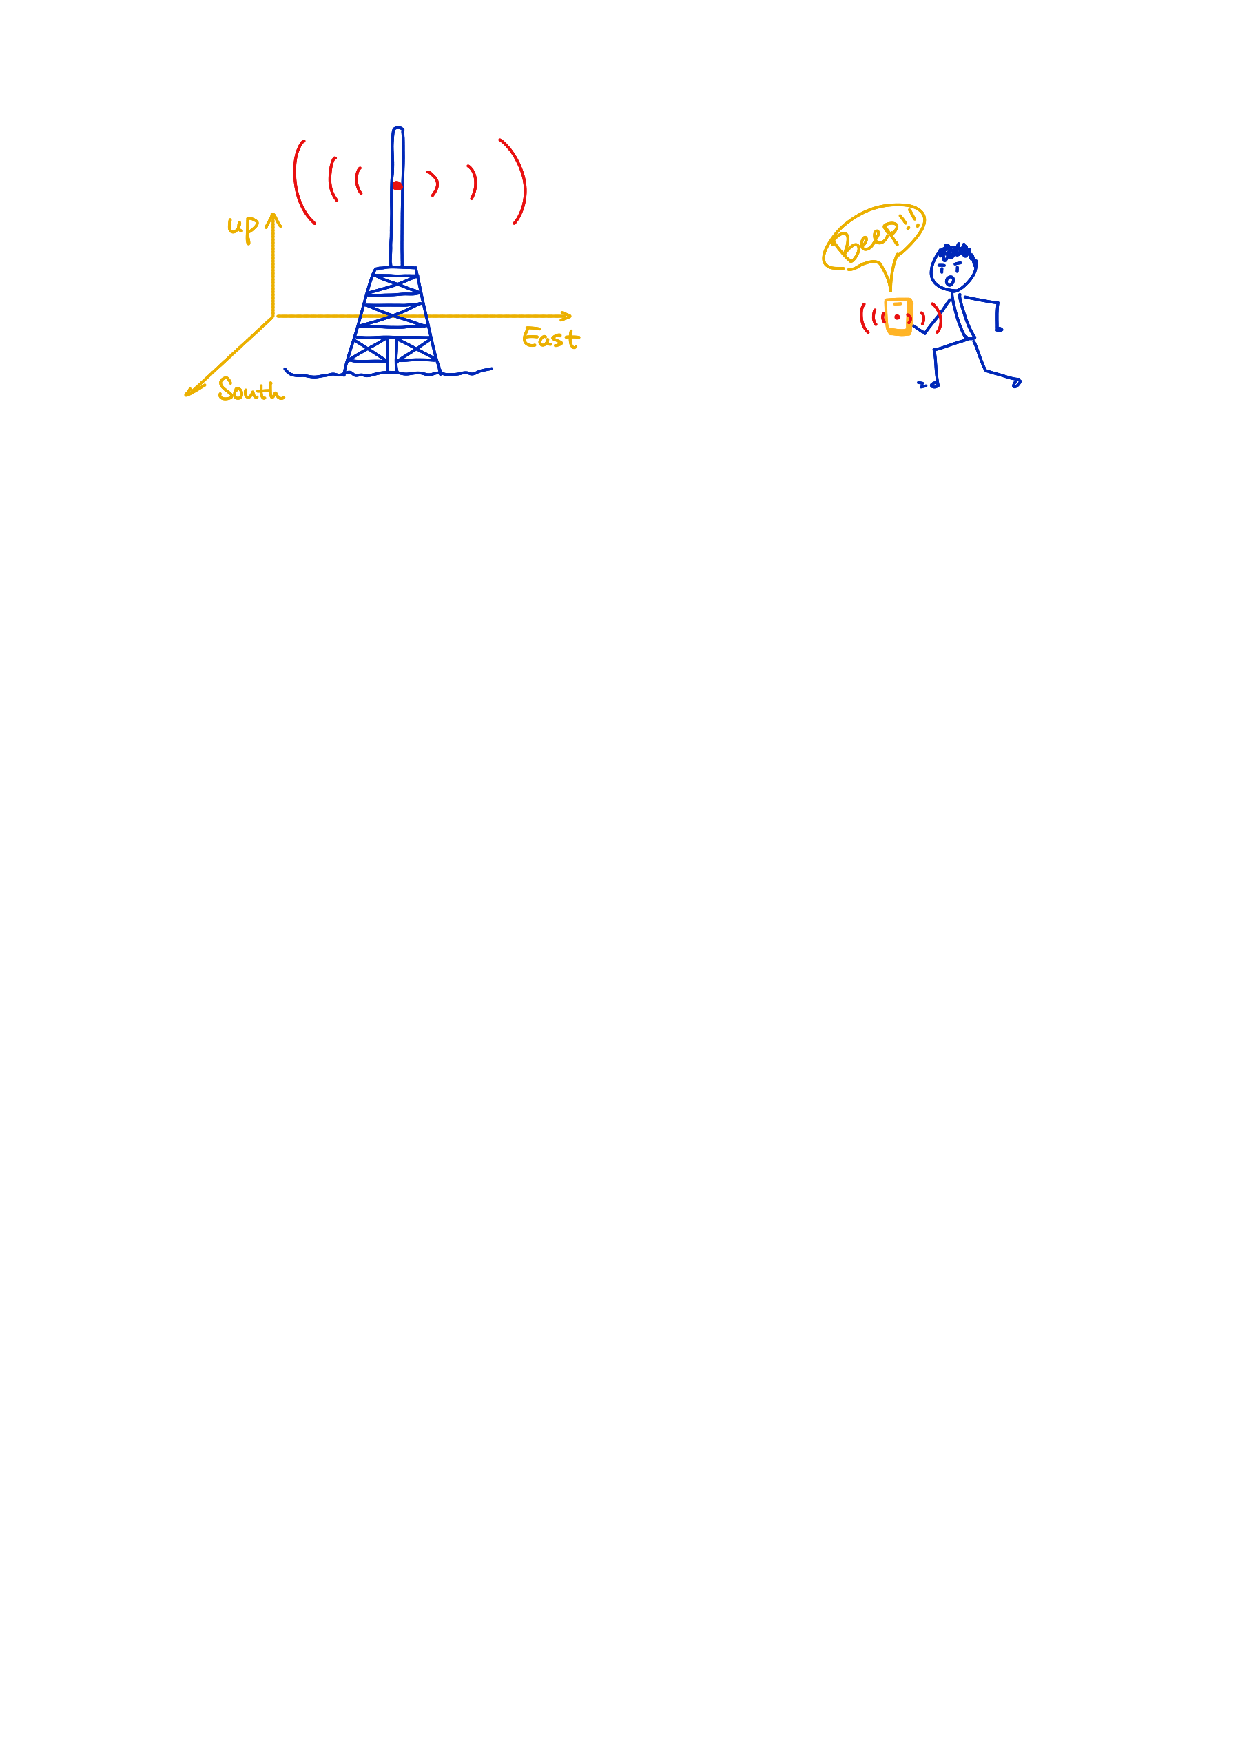
\includegraphics[scale=0.8]{antenna}
\end{center}

\noindent A ``$\perp$-mobile" antenna is emitting cell-phone signals. The antenna is oriented vertically, and it emits a signal that travels horizontally outward from the antenna. Jinyan is standing due east of the antenna, and at his location, the signal is traveling eastward. At one instant, Jinyan measures the electric field at his location and finds that the field is pointing straight up with magnitude $3\,$V/m.\\

\noindent\textbf{Part (a)} What are the direction (west? east? south? north? up? down?) and magnitude (numerical) of the magnetic field at Jinyan's location at that instant?\\


\noindent \textbf{Part (b)} The signal that Jinyan receives has a wavelength $\lambda = 1\,$m. If Jinyan's jPhone-13 is receiving a very steady signal throughout the time, find the direction and magnitude of electric field, and that of magnetic field at his location $\lambda/(2c)$ seconds after. \footnote{This is a challenging problem, but it turns out that you don't need to do any numerical computation here. You just need to figure out what I am asking, and recall some knowledge about waves.}\,\footnote{Using $c = \lambda f$ and $f = 1/T$, find $T$ in terms of $c$ and $\lambda$. Then determine what $\lambda/(2c)$ means.}\\

\noindent\textbf{Part (c)} In this part, treat the antenna as a point source emitting wave signal in all directions. If Jinyan is standing $1\,$km from the antenna and $3\,$V/m is the amplitude of the oscillating electric field at his location, estimate the intensity of the cell-phone signal emitted by the antenna at the location $1\,$m from the antenna.\\


\newpage
\noindent The measured electric field at Jinyan's location is polarized in the vertical direction.\\ 

\noindent\textbf{Part (d)} Jinyan then uses two polarizing sheets to change the polarization of the wave signal. The first one is oriented $\theta_1 = 30^\circ$ from the vertical, and the second one is oriented $\theta_2 = 90^\circ$ from the vertical. The two sheets are put one after another along the line of the wave transmission such that the wave signal will pass through the first one and then the second one. Find the intensity of the wave after it has passed through the second polarizer.\\

\noindent\textbf{Part (e)} Jinyan's evil friend Michael sneakily switched the order of the two polarizers in part (d). Now what intensity of the wave will Jinyan measure after the wave has passed through the second polarizer?

\newpage
\section*{Problem 1}
The key relation for an electromagnetic wave is that the direction of propagation is parallel to $\vec{E}\times \vec{B}$, and the magnitudes satisfy
\begin{align*}
E = cB\,.
\end{align*}
Here the wave is traveling eastward, and at the instant we care about, the electric field points upward with magnitude $3\,$V/m. In fact, in this story, the physical picture is as follows: In the little cartoon, the red dot in the antenna can be thought of as an electron moving up and down. The oscillation of the electron creates oscillation of the electric field (up and down), and oscillation of the magnetic field (north and south). That produces the propagation of an electromagnetic wave in the horizontal direction away from the antenna, and thus the signal is received by Jinyan.\\

For your reference, here are the different cases for the direction of propagation of electromagnetic waves. You can verify them using the right-hand rule. 
\begin{center}
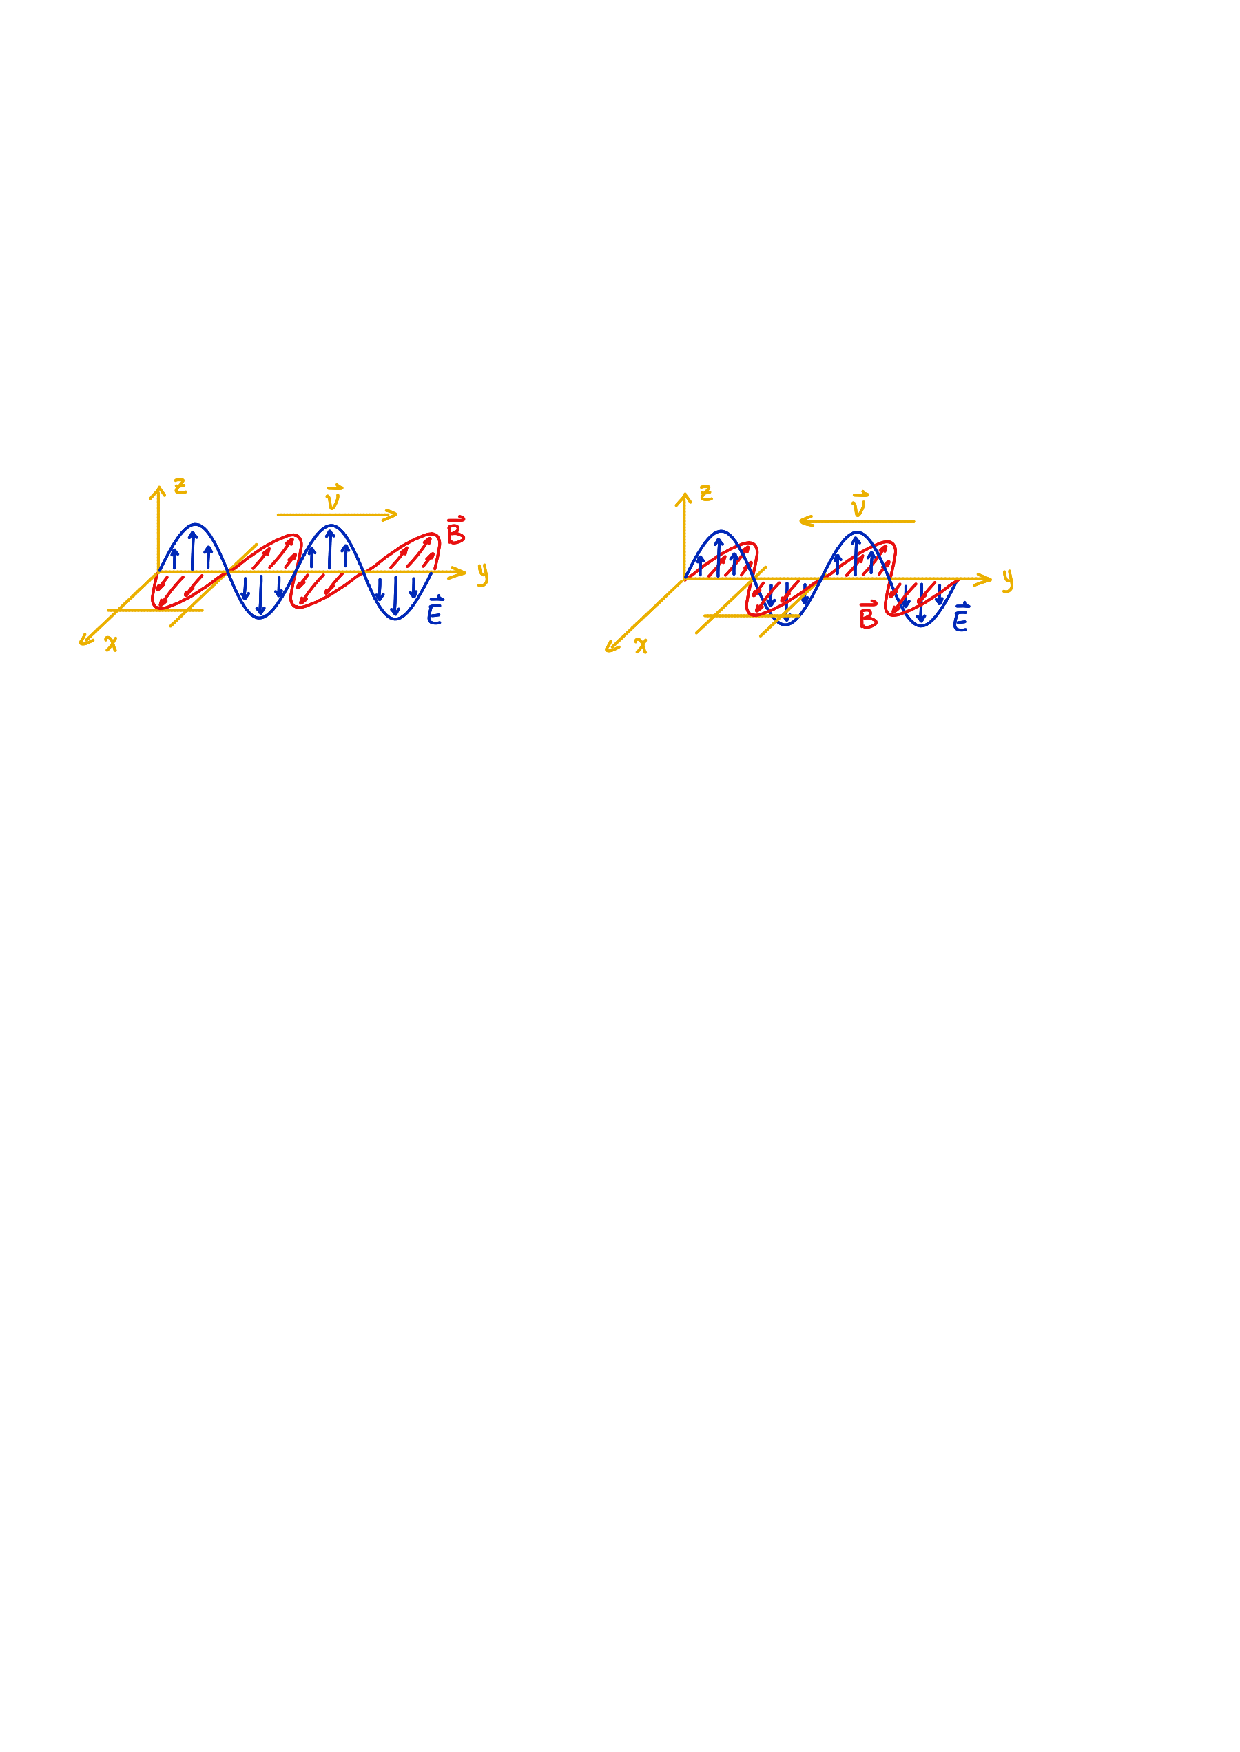
\includegraphics[scale=0.85]{waveDirection}
\end{center}


\noindent\textbf{Part (a)} We first find the magnitude of the magnetic field:
\begin{align*}
B = \frac{E}{c} = \frac{3\,\text{V/m}}{3\cdot 10^8\,\text{m/s}} = 1.0\cdot 10^{-8}\,\text{T}\,.
\end{align*}
Now we determine the direction. We want the cross product
$\vec{E}\times \vec{B}$
to point east. Since $\vec{E}$ points up, according to the right-hand rule, the magnetic field must point south in order for the cross product to point east. \\

\noindent\textbf{Part (b)} Using
\begin{align*}
c = \lambda f\,,\qquad f=\frac{1}{T}\,,
\end{align*}
we find the period of the wave
\begin{align*}
T = \frac{\lambda}{c}\,.
\end{align*}
Therefore, half of the period is 
\begin{align*}
\frac{\lambda}{2c} = \frac{T}{2}\,.
\end{align*}
So the question is asking what happens half a period later. Half a period later, an oscillating wave reverses the direction of both $\vec{E}$ and $\vec{B}$, while keeping the same magnitude. Therefore, at time $\lambda/(2c)$ seconds later, $
\vec{E} \text{ points down, with magnitude } 3\,\text{V/m}\,,$ and $
\vec{B} \text{ points north, with magnitude } 1.0\cdot 10^{-8}\,\text{T}\,.$
This makes sense: both fields reverse direction, but the wave still propagates eastward because
\begin{align*}
\vec{v}\parallel (-\vec{E})\times (-\vec{B}) = \vec{E}\times \vec{B}\,.
\end{align*}

\noindent\textbf{Part (c)} We first find the intensity at Jinyan's location. For a sinusoidal electromagnetic wave with electric-field amplitude $E_0$, the average intensity is
\begin{align*}
I = \frac{1}{2}\epsilon_0 cE_0^2\,.
\end{align*}
The factor $1/2$ comes from averaging the square of the oscillating electric field over a full period. Here $E_0=3\,$V/m, $c=3.0\cdot 10^8\,$m/s, and $\epsilon_0=8.85\cdot 10^{-12}\,$F/m. Therefore, at a distance of $1\,$km from the antenna, the intensity is
\begin{align*}
I
&=\frac{1}{2}(8.85\cdot 10^{-12}\,\text{F/m})(3.0\cdot 10^8\,\text{m/s})(3\,\text{V/m})^2\\
&\approx 1.19\cdot 10^{-2}\,\text{W/m}^2
\approx 1.2\cdot 10^{-2}\,\text{W/m}^2\,.
\end{align*}
Next we estimate how the intensity changes with distance. As the wave travels outward, the same power is spread over an area proportional to $r^2$. Therefore, the intensity obeys the inverse-square relation
\begin{align*}
Ir^2=\text{constant}\,.
\end{align*}
Let $r_{\text{far}}=1\,\text{km}=1000\,$m and $r_{\text{near}}=1\,$m. Then
\begin{align*}
I_{r_{\text{far}}}r_{\text{far}}^2
&=I_{r_{\text{near}}}r_{\text{near}}^2\,,
\end{align*}
from which we have
\begin{align*}
I_{r_{\text{near}}}
&=I_{r_{\text{far}}}\left(1000/1\right)^2\approx(1.19\cdot 10^{-2}\,\text{W/m}^2)(10^6)=1.19\cdot 10^4\,\text{W/m}^2\,.
\end{align*}
Thus, neglecting absorption and treating the antenna as a source whose radiation spreads outward, the estimated signal intensity at $1\,$m is $1.19\cdot 10^4\,$W/m$^2$.\\

\noindent\textbf{Part (d)} Before the wave reaches the first polarizer, its electric field is polarized vertically. The intensity transmitted through an ideal polarizer is described by Malus's law,
\begin{align*}
I_{\text{out}}=I_{\text{in}}\cos^2(\theta)\,,
\end{align*}
where $\theta$ is the angle between the polarization direction of the incoming wave and the transmission axis of the polarizer. The polarizers are at Jinyan's location, so the incident intensity is the intensity at $1\,$km that we calculated as the first step in part (c),
\begin{align*}
I_0\approx 1.19\cdot 10^{-2}\,\text{W/m}^2\,.
\end{align*}
The incoming wave is polarized vertically, while the first polarizer is oriented $30^\circ$ from the vertical. Therefore,
\begin{align*}
I_1
&=I_0\cos^2(30^\circ)
=\frac{3}{4}I_0\,.
\end{align*}
After passing through the first polarizer, the wave is polarized along the first polarizer's axis, which is $30^\circ$ from the vertical. The second polarizer is $90^\circ$ from the vertical, so the angle between the polarization entering the second polarizer and its transmission axis is
\begin{align*}
\Delta\theta=90^\circ-30^\circ=60^\circ\,.
\end{align*}
Applying Malus's law again gives
\begin{align*}
I_2
&=I_1\cos^2(60^\circ)
=\left(\frac{3}{4}I_0\right)\left(\frac{1}{2}\right)^2\approx 2.2\cdot 10^{-3}\,\text{W/m}^2\,.
\end{align*}
Therefore, the intensity after the wave has passed through the second polarizer is approximately $2.2\cdot 10^{-3}\,$W/m$^2$.\\

\noindent\textbf{Part (e)} After Michael switches the order, the polarizer oriented $90^\circ$ from the vertical comes first. The incoming wave is vertically polarized, so the angle between its polarization and the first transmission axis is $90^\circ$. Malus's law gives
\begin{align*}
I_1'=I_0\cos^2(90^\circ)=0\,.
\end{align*}
No wave intensity remains after the first polarizer. Consequently, placing the polarizer oriented $30^\circ$ from the vertical second cannot restore the wave,
\begin{align*}
I_2'=I_1'\cos^2(60^\circ)=0\,.
\end{align*}
Therefore, after the order of the two polarizers is switched, Jinyan will measure an intensity of $0\,$W/m$^2$ after the second polarizer. From here we see that the order of placing the polarizers does matter. \\


\vfill

\begin{center}
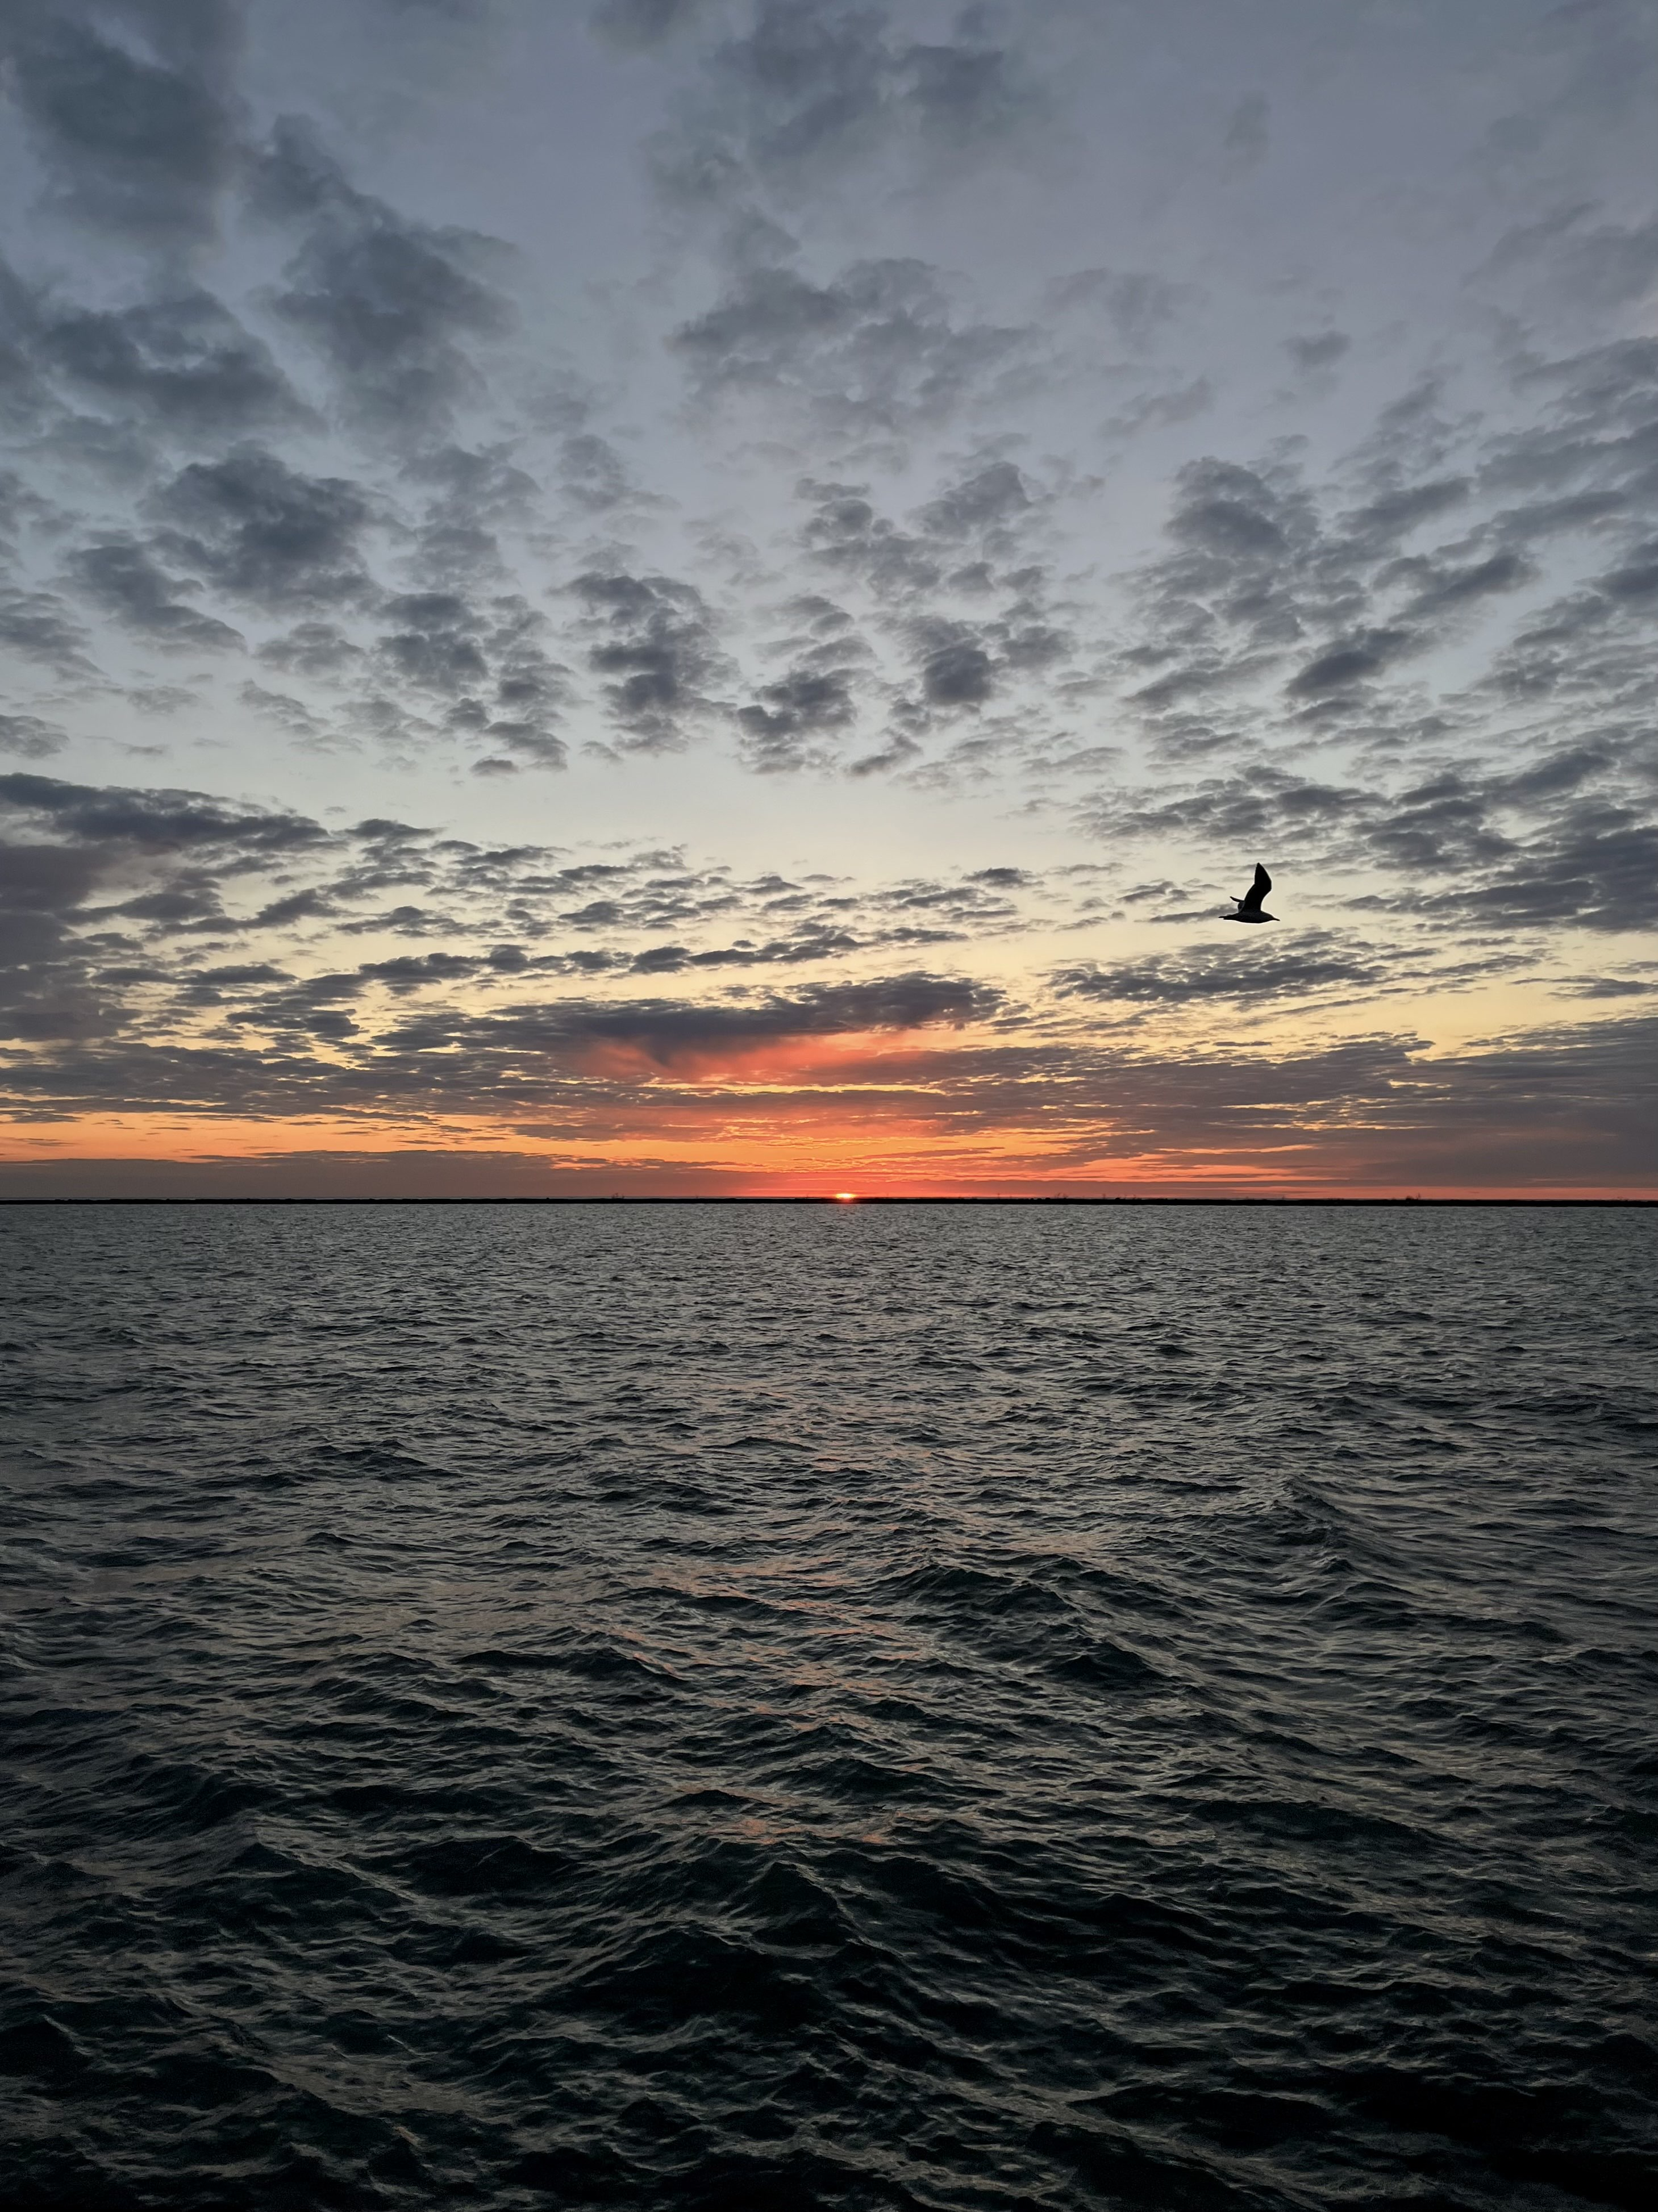
\includegraphics[scale=0.135]{michgiganLake}\\
\hfill\break
Another sunrise at Lake Michigan at Chicago, IL. Pictured in March 2026.\\
\end{center}

\end{document}
